% THESIS CHAPTER

\chapter{Landing on a mobile platform}
\label{chap:seventh}
\ifpdf
    \graphicspath{{Chapter7/Figures/PNG/}{Chapter7/Figures/PDF/}{Chapter7/Figures/}}
\else
    \graphicspath{{Chapter7/Figures/EPS/}{Chapter7/Figures/}}
\fi

% short summary of the chapter
\section*{Summary}

This chapter concerns the task of landing on a platform of arbitrary height while it is moving on the horizontal plane. After a brief introduction to the topic and the statement of general assumptions, the experimental setup is described. Later on the solution to the problem is presented and the control algorithm described. Last section presents and comments experiment results.

\section{Brief Introduction}


The problem of landing on a moving platform presents different technical and theoretical challenges. The origin of this research trend is found in the military field especially within the navy. Air carriers became a reality a number of years ago and engineer found different methods to land and take of from the platform. The main issue an aircraft face during landing on a sea based platform is the effect of waves movement of the boat. But still landing is made by a human pilot. Regarding MAVs, a bunch of people built home made robot-quadrotor platforms able to cooperate (see figure \ref{figure:couple}).
\begin{figure}[h]
\centering
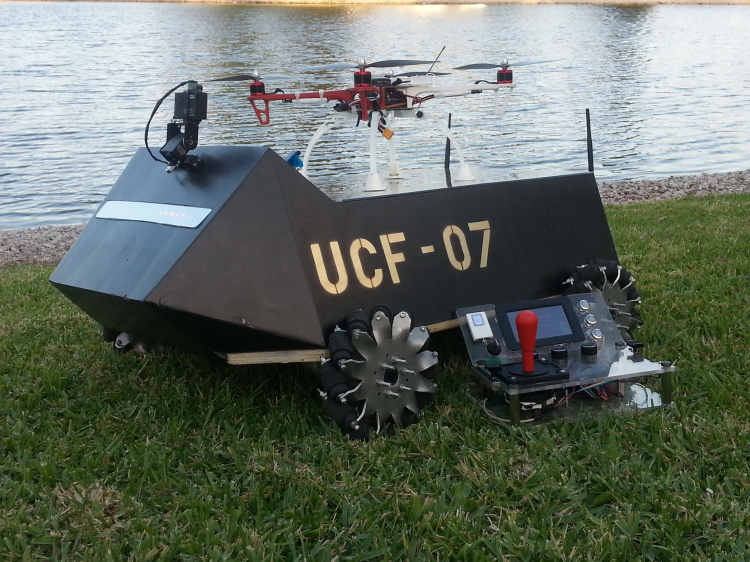
\includegraphics[width = 0.6\textwidth ]{couple.jpg}
\label{figure:couple}
\caption{Home made cooperative platform/quadrotor project}
\end{figure}

A very ambitious project is being pursued by SpaceX, an american aerospace manufacturer and space transport services company. What the want to achieve is a new reusable space program in which the first stage of a rocket, one detached, returns back to surface in an autonomous way. The key aspect is that the stage must land on a floating platform on the ocean (figure \ref{figure:spacex}). 
\begin{figure}[h]
 \centering
   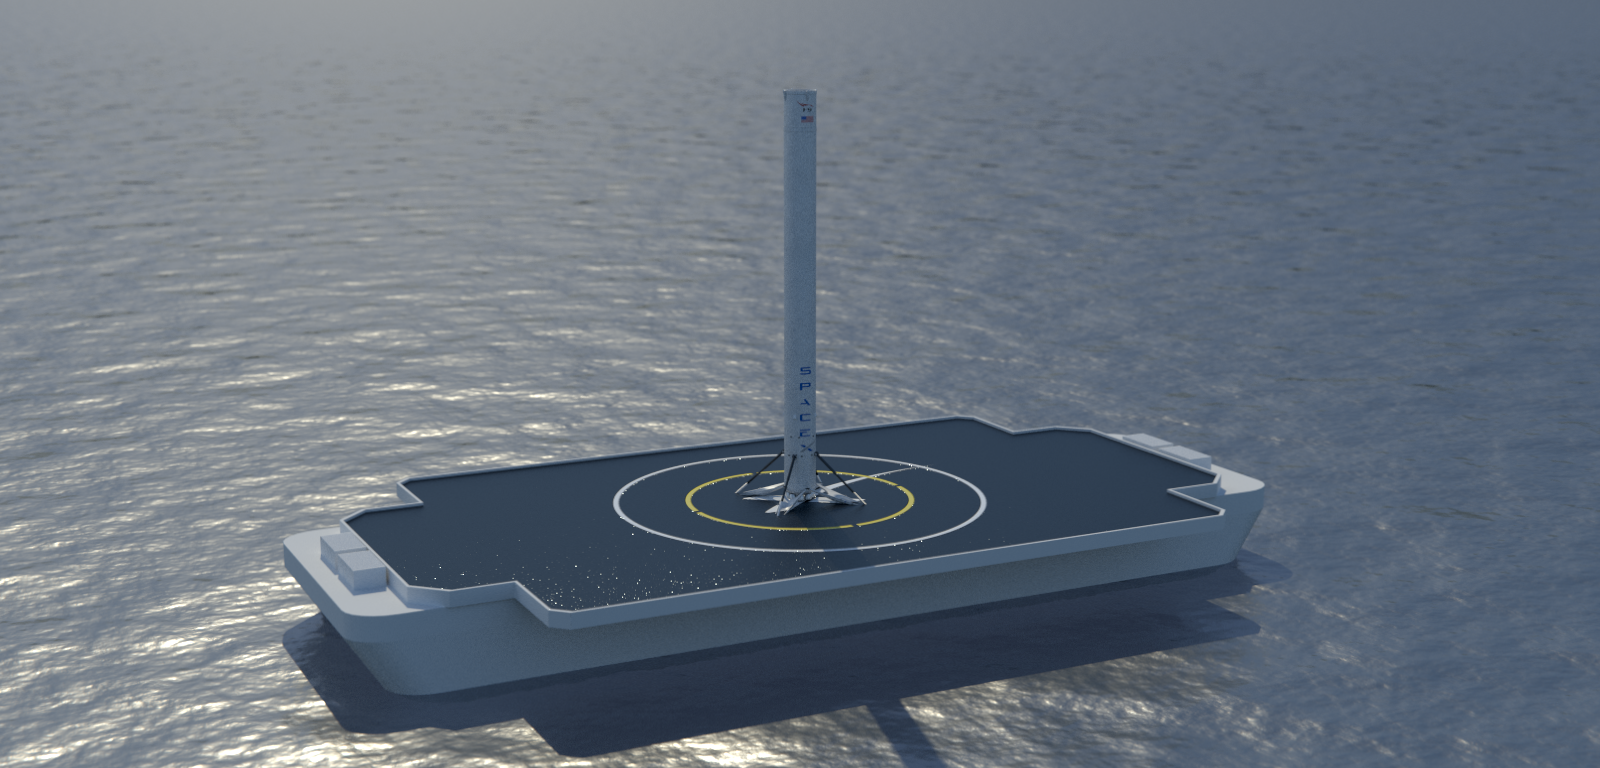
\includegraphics[width = 0.6\textwidth ]{spacex.png}
    \caption{Prototype of the SpaceX platform with rocket.}
   \label{figure:spacex}
\end{figure}

This ongoing research from different entities emphasizes the fact that the following problem is still open, thus there could space for future exploration. 

Coming back to our case, at this point we have available a working architecture which controls through position and yaw, set points the IRIS. Thus we may ask the following statement:	

\paragraph{Problem statement} It is possible, through position control, to develop an algorithm which is able to guide IRIS along a landing maneuver on a mobile platform? \newline

\noindent
During my work I proved that this objective is achievable, at least under a number of assumptions.

\subsection{General assumptions}

The entire task has been carried out under certain assumptions which simplifies the development of the solution but still maintain a certain level of consistency. 

The assumptions under which the system is constrained are:
\begin{itemize}
\item Only the position of the platform is know, velocity is not used in the controller.
\item The trajectory of the platform is assumed to be mostly linear, no sudden changes in direction are taken into account.
\item The velocity of the platform is constant.
\item The point where the robot changes direction, because of the size  of the lab, is roughly known.
\end{itemize}
Those conditions are a good point to start with since they are quite close to reality. The linear and constant velocity assumptions are reasonable, different practical examples fall in this case. Imagine a car moving on a highway, a boat in the ocean or a mobile robot exploring the environment. Those vehicles have similar dynamics to the one described.

\section{Experimental setup}
The equipment used for the design and experimentation consists in a mobile robot with a cardboard platform attached to the top. The robot is called labmate, an old platform which features two motor installed in a differential fashion, two 12V batteries and a plastic cover for the chassis. Four markers are placed on the top to corners of the platform, in this way the center of mass of the rigid body lies at the center of the landing area. Figure \ref{figure:labmate} shows the mobile robot with the four markers on. 
\begin{figure}[h]
 \centering
   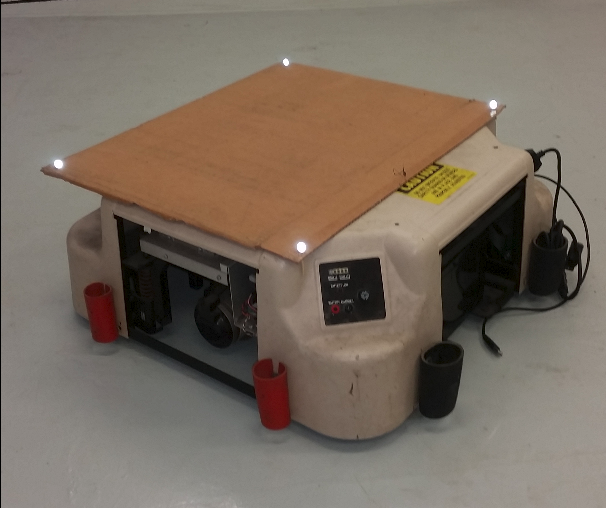
\includegraphics[width = 0.6\textwidth ]{labmate.png}
    \caption{Labmate mobile robot.}
   \label{figure:labmate}
\end{figure}
The designed experiment consists in landing on the platform while it is moving on a straight line back and forth. We programmed the labmate to move to the front till 2.4 meters and then back in a straight line with fixed speed. The robot path coincides with the diagonal of the room in order to take advantage of the longer distance. 

The robot is controlled by a computer placed on board within a Linux environment. Through serial port, the computer is able to send commands to the robot which executes them. An application that manages the communications with the labmate was developed years ago in the university of Genova. In order to run the modules, ssh protocol is used to manage the starting of the robot from remote. 

Moreover, since the experiment takes place in a close and controlled environment, the labmate at a certain point changes abruptly direction going to the opposite way. This goes against one of the assumptions but the problem is avoided. We assume to know the external points of the path, then when the robot approaches those location we can inhibit the landing procedure prevent the danger of landing when the platform changes direction.  Thus, we define a landing window, along the path, on which the robot can perform the landing operation. Outside the window, the robot will raise to a maximum height. Figure \ref{figure:window} shows the geometry of the experiment. The diagonal path has colored segments. The green segment represent the landing window, while the red segments are the prohibited sections. The landing window is approximately 1 meter long. 
\begin{figure}[h]
 \centering
   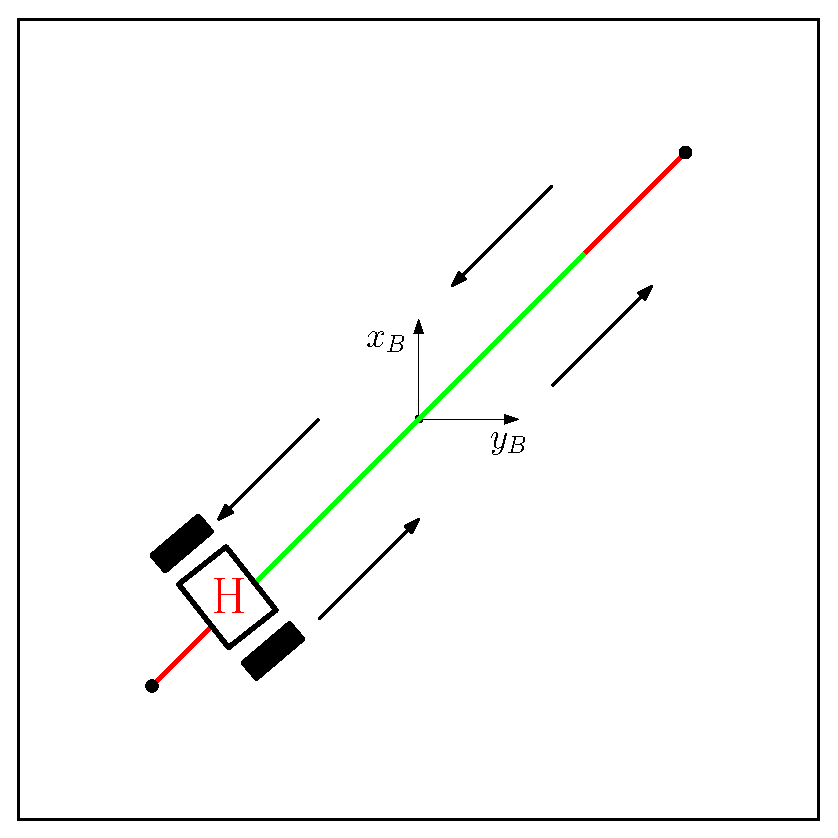
\includegraphics[width = 0.8\textwidth ]{landwindow3.eps}
    \caption[Experiment geometry]{Moving platform defined by H. Green is landing window while red are prohibited segments.}
   \label{figure:landwindow}
\end{figure}


\section{Tracking and landing}
This section describes the techniques involved in the designing of a method to accomplish the task.

First we divide the problem in two subproblems, in fact vertical and horizontal dynamics are decoupled and treated separately. This is a common practice in system design. 

The first treated part is tracking. By \textbf{tracking} we mean the act of forcing the output signal of the system to a reference signal and minimizing the error between the two. Applied to this case, we can refer to the output signal $\boldsymbol{P_r}$ as the 2-D horizontal position of the center of mass of the robot. The tracking reference signal 
$\boldsymbol{P_t}$ is defined as the horizontal 2-D position  of the platform center of mass. Both signals are provided as feedback from the mocap and acting on the inputs (position set points) with a suitable control law, one should minimize the error.

\paragraph{Tracker design} I would like to stress out the fact that the only way we can act on the system is by issuing position set points $\boldsymbol{P_{sp}}$. They could be coincident with the target or not, it depends on the control law. Let us consider a 2-D position set point for now.

With an initial guess we may design the first controller by setting set point equal to the target which may be logical. Chapter \ref{chap:fifth} exploits a position controller designed in order to track position set points, thus it seems reasonable to proceed in this way. Hence the very first design is of the form:
\begin{equation}
\boldsymbol{P_{sp }} = \boldsymbol{P_{r}}
\label{eq:contr1}
\end{equation}
This control law is very simple but useless. Despite of what one may think, this approach will never work properly for a moving target. The gains of the controllers are not infinite and the response to a command is not immediate. The transient time adds delay resulting in the robot following the platform but not aligning properly with it. Is more or less like running after someone but never actually catching him.

Figure \ref{figure:nogain} represents an actual trial in the lab. The implemented control law is the one explained in \ref{eq:contr1} while the purpose of the experiment was to qualitatively evaluate the position error. In this particular situation, the platform is moving with a velocity $\boldsymbol{V_t}$ to the left and the robot is following with a velocity $\boldsymbol{V_r}$. We can observe a position error vector $\boldsymbol{P_e}$ between the two vehicles approximately constant at steady state and with a variable module depending on the relative robot speed.
\begin{figure}[h]
 \centering
   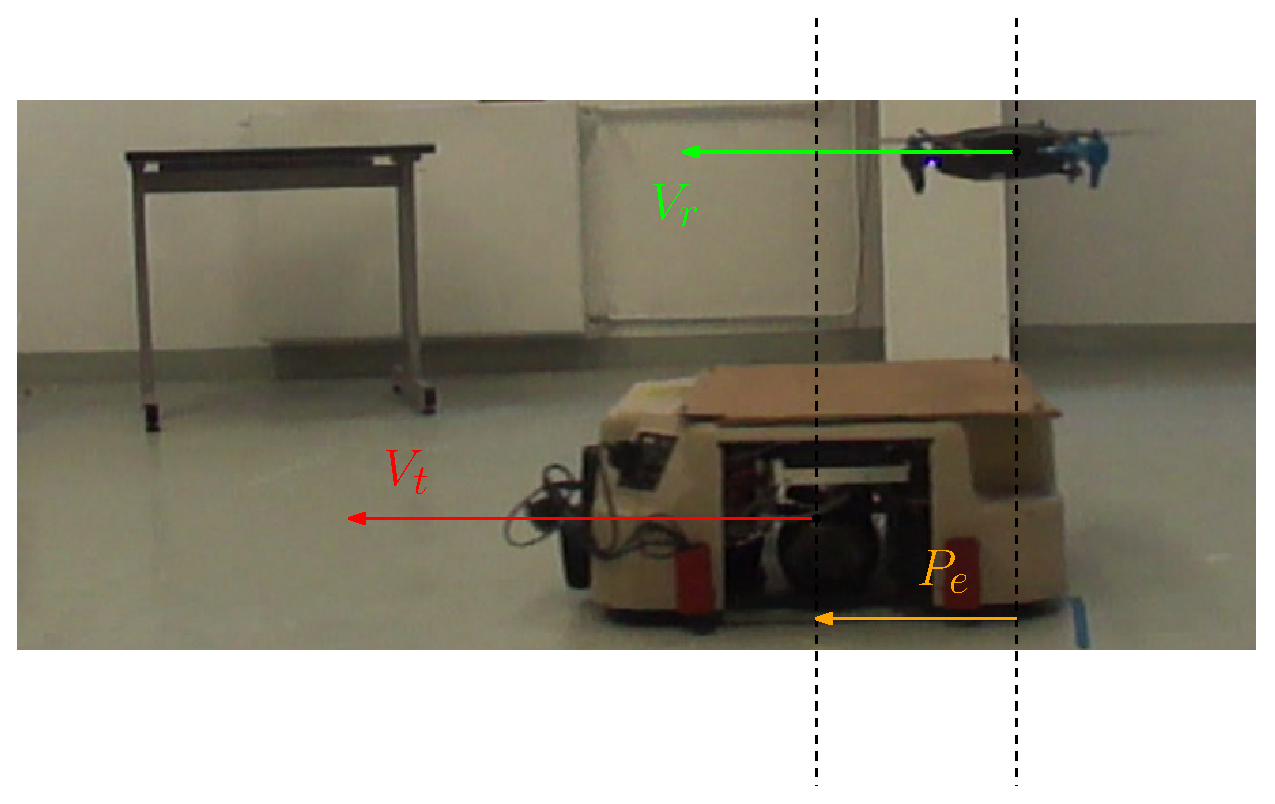
\includegraphics[width = 0.8\textwidth ]{tracknogain2.eps}
    \caption[Tracking with no gain]{Tracking of the moving platform by following its position. A static error appears.}
   \label{figure:landwindow}
\end{figure}
The control can be improved by adding  another source for feedback, the position error which can be measured by $\boldsymbol{P_e} = \boldsymbol{P_{t}} - \boldsymbol{P_{r}}$. By observing the phenomenon we can think of issuing a position set point a bit ahead the robotic platform so that, even if the robot does not converges to $\boldsymbol{P_{sp}}$, we can in some way anticipare the platform. That said, the controller is modified to the following:
\begin{equation}
\boldsymbol{P_{sp}} = \boldsymbol{P_{r}} + K_p \boldsymbol{P_e} \boldsymbol{P_{r}}
\label{eq:contr2}
\end{equation}
Meaning that, depending on the actual horizontal error, the set point is accordingly issued, weighted by $K_p$ gain and placed ahead the mobile platform. 

This is a big improvement but it is still insufficient. Proportional controls are made to work with the presence of errors. If the target is reached, the error goes to zero and the equation \ref{eq:contr2} simply becomes \ref{eq:contr1}. As stated befor, the error is static, meaning that at regime it is constant. The best way to compensate for this kind of errors is to insert and integral action. Hence the third and final controller is:
\begin{equation}
\boldsymbol{P_{sp}} = \boldsymbol{P_{r}} + K_p \boldsymbol{P_e} +  K_i \int \boldsymbol{P_e}
\label{eq:contr3}
\end{equation}
Integrating the error, the last terms grows. When the robot reaches the vertical of the platform, proportional term goes to zero but the integral remains at a certain value. This value it is somehow related to the velocity of the platform and it is able to cancel static error.

There are drawbacks to this approach. When the platform suddenly changes direction, the integral is saturated and lead to an overshoot. One possible solution is to reset the integral every time a sudden motion is detected.

\paragraph{Landing}

At this moment, the tracking problem is solved. A way to safely land on the platform must be designed. Moreover, the procedure should be robust enough to detect horizontal error and decide whether land or not. In this case I used a very simple but surprisingly effective method. 

Let us consider just the vertical dynamics and forgot about the rest. The goal is to decrease the height in order to approach the platform and land without missing. The parameter which gives an idea on how it is safe to land is the horizontal distance to the robot, namely $\lVert \boldsymbol{P_e} \rVert = d$. Depending on the value of d, the robot may decide to land or go up. Thus, the involved variables are the vertical set point $z_{sp}$ and the horizontal distance $d$. 

The relation between distance and set point are many and up to designer. I used the simplest curve one may think, the line. A linear relationship between $z_{sp}$ and $d$ is used. Let 


\section{Experimental results}

